\chapter{Results}
\label{ch:results}

This chapter examines the results achieved through our experimental work.
Starting off we will show the resulting models through pyLDAvis in section \ref{results:pyldavis}. The topics are evaluated and compared with a coherence score in section \ref{results:coherence}. The tables show multiple topics with their top terms in section \ref{results:topics}. The document distribution based on most relevant topic after applying the model on the corpus in section \ref{results:doc_distribution}. Ending with a silhouette coefficient score for the models in  section \ref{results:silhouette}. The models were generated using the gensim package and the results compare the train, test and held out data where applicable. 



\section{Model results}\label{results:modelresults}
Our results are created and evaluated with multiple aspects in mind. The human interpretation and semantic analysis of the documents have been leading for our models and results. Each section discusses one of these aspects. The experiments are conducted with the gensim package. The models have been created with 2 till 38 topics. The default settings in gensim allowed our models to be trained on our test and train data, further explained in section \ref{methodology:model_building}. 

\FloatBarrier
\section{Wordcloud}\label{results:wordcloud}
We represented our terms in a wordcloud, Fig \ref{fig:worldcloud}, which as the name implies simply shows the terms in the topics created by our models in a cloud. Nothing special so far to behold, but a quick glance on the words show words which are very domain specific as such we can not easily interpret the meaning behind the words or their relation.

 \begin{figure}[h]
    \centering
    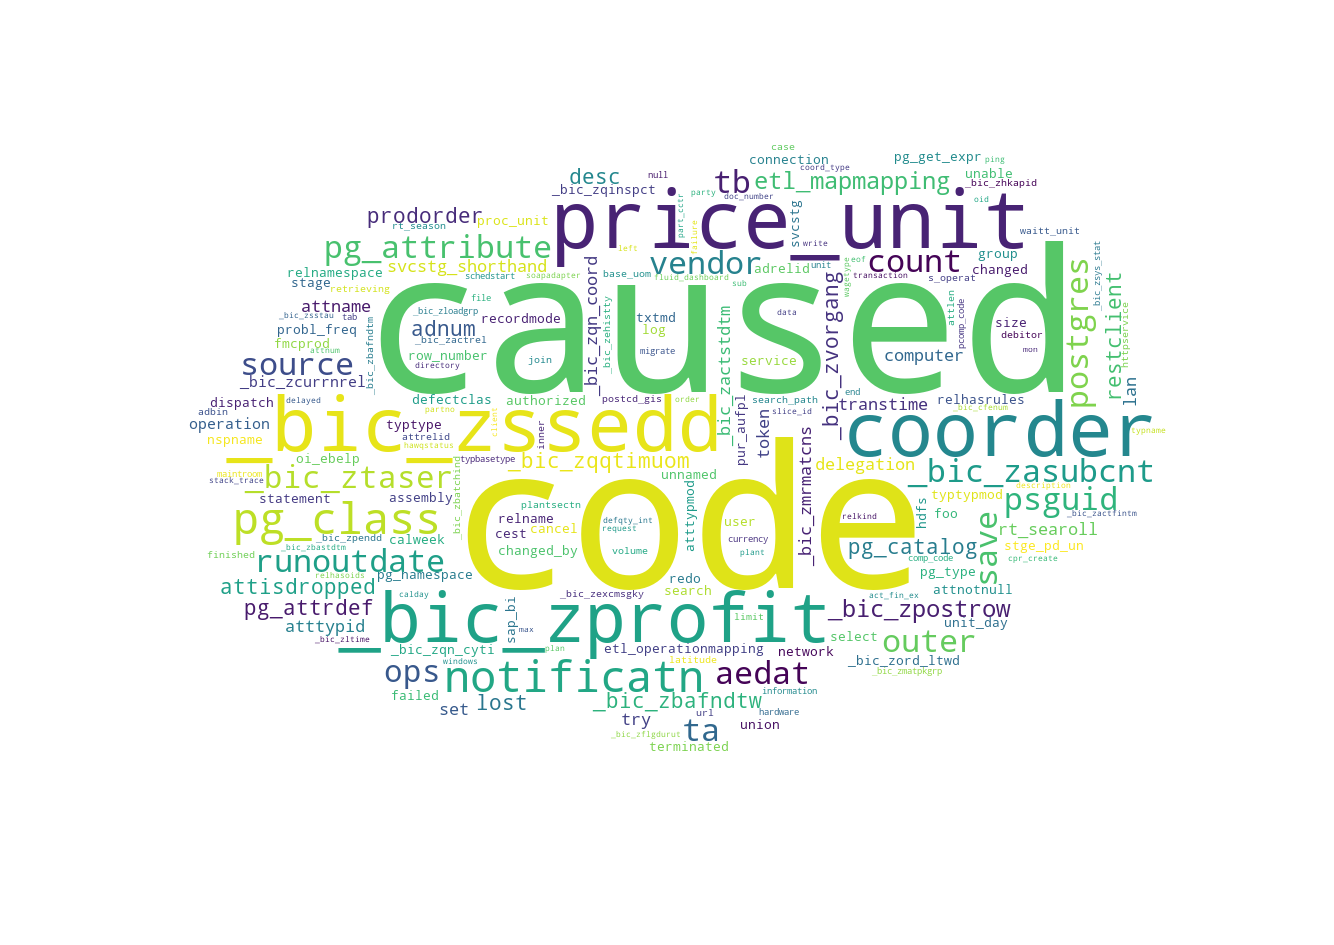
\includegraphics[width=15cm, height=8cm]{figures/wc.png}
    \caption{A wordcloud containing terms found in clusters}
    \label{fig:worldcloud}
\end{figure}

\FloatBarrier

\section{Topic overview}\label{results:topics}
First we examine the latent topics our models have generated based. We showcase the topic count 2, 5 and 10. We will use these as a reference for further topics. 
The remaining topics can be found in the appendix A \ref{appendices:modelgeneratedtopics}. 

If we keep our domain to recognising topics which could result in an error, we might deduce topics from our table \ref{tab:2topicsmodel}, \ref{tab:5topicsmodel}. \ref{tab:10topicsmodel}. 

\begin{table}[h]
\centering
\begin{tabular}{|l|l|l|l|l|l|}
 \hline
 Topic & Terms & & & & \\
 \hline
 \hline
 0 & user & information & retrieving & ta & select\\ 
 \hline 
 1 & failed & code & request & restclient & ping\\ 
 \hline 
\end{tabular}
\caption{Topic 1..2 with top 5 terms}
\label{tab:2topicsmodel}
\end{table}

Examining table \ref{tab:2topicsmodel}, we can not simply deduce what these two topics are about. We can at best say that the second topic is probably an error topic based on the simple word failed. So far the analyse is based on the sentiment rather on the semantic.


\begin{table}[h]
\centering
\begin{tabular}{|l|l|l|l|l|l|}
 \hline
 Topic & Terms & & & & \\
 \hline
 0 & ta & select & f & group & plan\\ 
 \hline 
 1 & fluid\_dashboard & text & tblasset\_ser & tbljob\_sow & group\\ 
 \hline 
 2 & v & r & order & null & tb\\ 
 \hline 
 3 & failed & code & request & source & restclient\\ 
 \hline 
 4 & user & information & retrieving & log & party\\ 
 \hline 
\end{tabular}
\caption{Topic 1..5 with top 5 terms}
\label{tab:5topicsmodel}
\end{table}

We continue on to our next table, table \ref{tab:5topicsmodel}. We see similar words in this table as table \ref{tab:2topicsmodel}, topic 3 and 4 have the same terms as topic 0 and 1 in the first table. Making it probable that these are common occurrences throughout our corpus. 
 
\begin{table}[h]
\centering
\begin{tabular}{|l|l|l|l|l|l|}
 \hline
 Topic & Terms & & & & \\
 \hline
 0 & request & migrate & restclient & url & ping\\ 
 \hline 
 1 & fluid\_dashboard & text & tblasset\_ser & tbljob\_sow & coord\_type\\ 
 \hline 
 2 & ordcateg & cancel & token & postgres & \_bic\_zpmrsord\\ 
 \hline 
 3 & orderitem & redo & record & unit\_day & length\\ 
 \hline 
 4 & f & foo & count & ta & v\\ 
 \hline 
 5 & ops & hawqstatus & down\_indic & set & \_bic\_zlongit\\ 
 \hline 
 6 & request & ping & migrate & url & http\\ 
 \hline 
 7 & failed & material & recordmode & notificatn & group\\ 
 \hline 
 8 & ta & select & group & plan & dispatch\\ 
 \hline 
 9 & user & information & retrieving & tblasset\_ser & tbljob\_sow\\ 
 \hline 
\end{tabular}
\caption{Topic 1..10 with top 5 terms}
\label{tab:10topicsmodel}
\end{table}

The final table we will manually inspect is table \ref{tab:10topicsmodel}. The more topics we see the harder it is to recognise topics each term distribution represents. 

Trying to infer topics through the top terms can not be done well this way. Servers logs which are created for domain specific programs and systems make it harder to interpret a coherent and distinctive topic. Noticably in higher topic counts is the amount of similar top terms, e.g. term 'ta' in the model with 11 topics appears 3 times as top term in 3 seperate topics. This might simply be a popular word for multiple documents or the model is not sufficient. The results so leave us with not much. 

\FloatBarrier
\section{Comparison of the infered topics through pyLDAvis}\label{results:pyldavis}
As mentioned before at \ref{methodology:humanperception}, Pyldavis already includes the distance metric Jensen Shannon and as such computes distance of each topic. The topics have been clustered using the term relevance. It does not show the reality of the documents being clustered, only an estimate of the size compared to other clusters based on the term frequency. Referencing \ref{appendices:pyldavis} we created multiple figures to compare. This allows us to see if the models have been trained well enough to create distinct topics.

\begin{figure}[h]
    \centering
    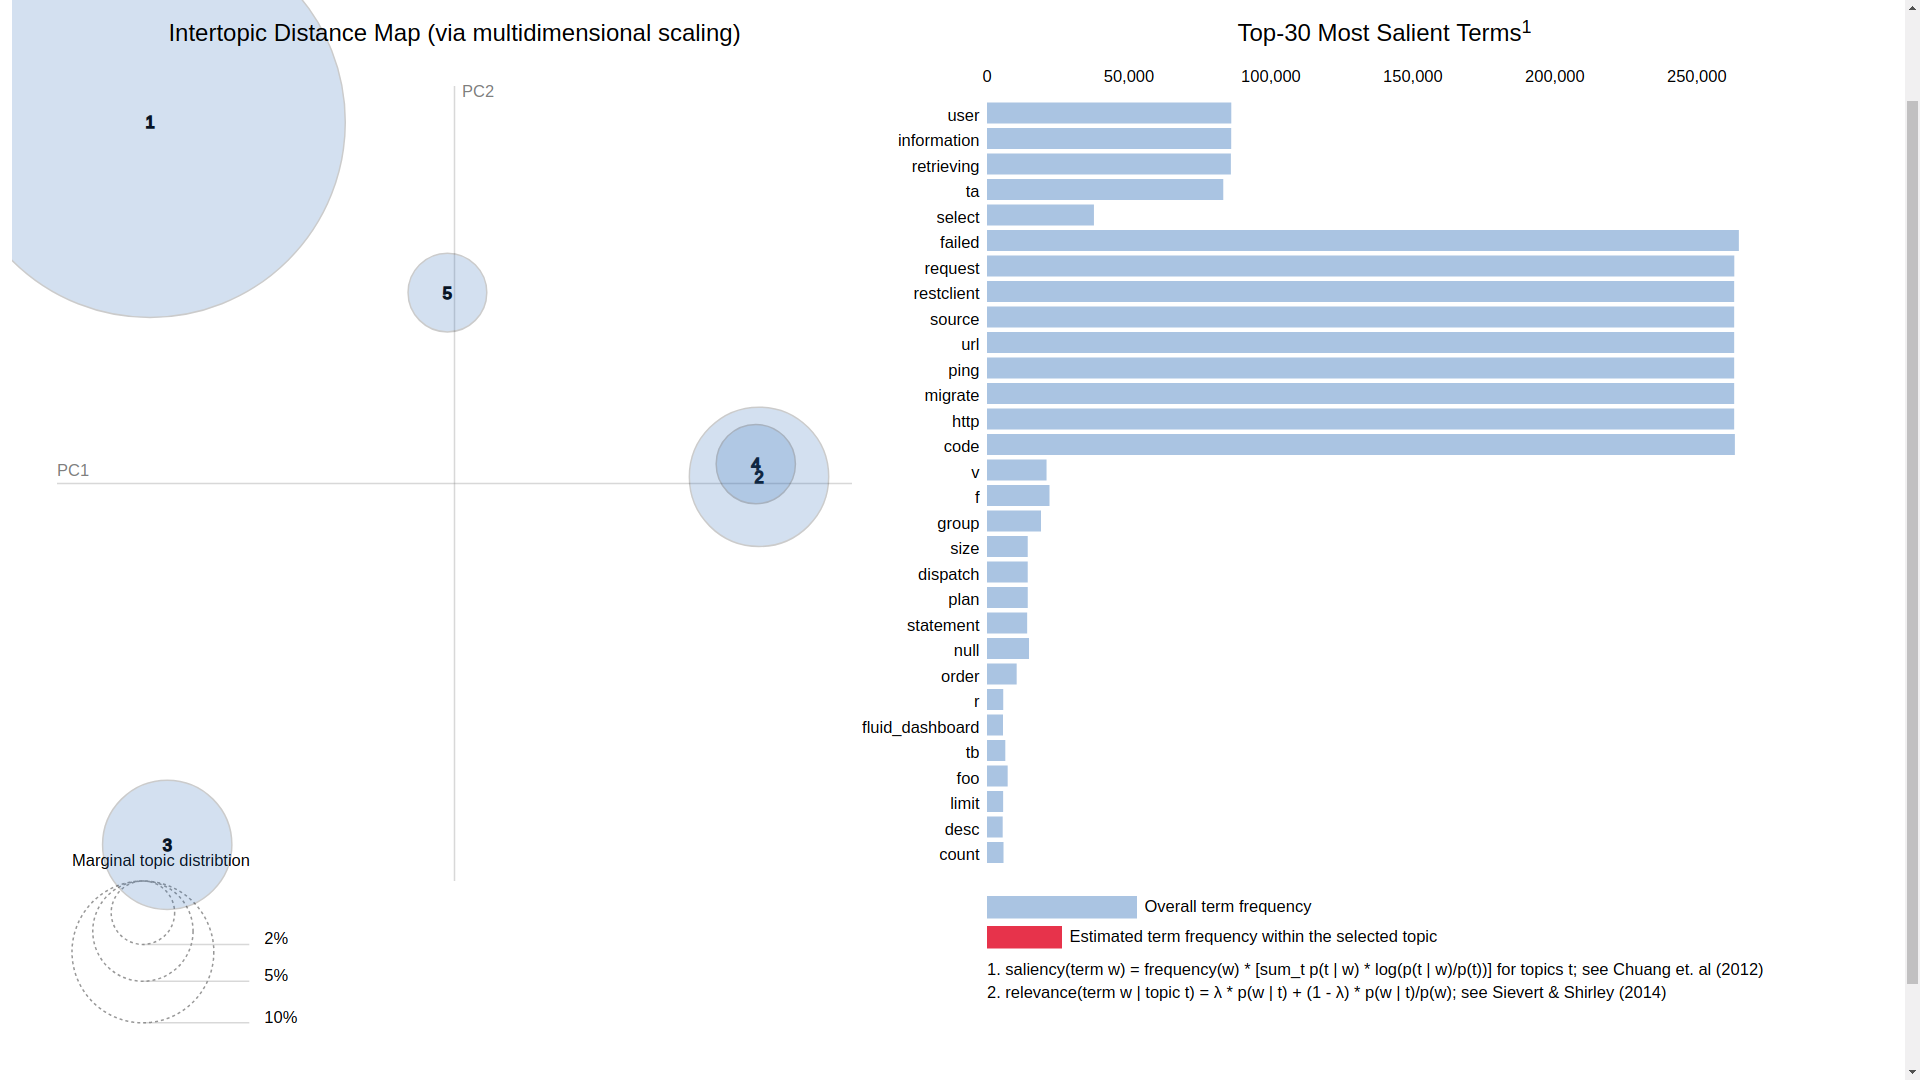
\includegraphics[width=15cm, height=8cm,trim=0 0 100px 0, clip=true]{figures/pyldavis/pyldavis_5.png}
    \caption{PyLdavis topic visualisation with 5 topics}
    \label{fig:pyldavis_5}
\end{figure}

For simple reference we use Fig \ref{fig:pyldavis_5} to compare other generated pyLDAvis distance maps. Interestingly the figure implies that there is already an overlap of topics with as few as 5 topics. Topics 2 and 4 are already overlapping, this could simply be a result of the dimensional reduction applied by pyLDAvis. The remaining topics have a clear distance from each other. Although topic 1 is very large, it is expected though because the dataset contained a lot of similar documents.

\begin{figure}[h]
    \centering
    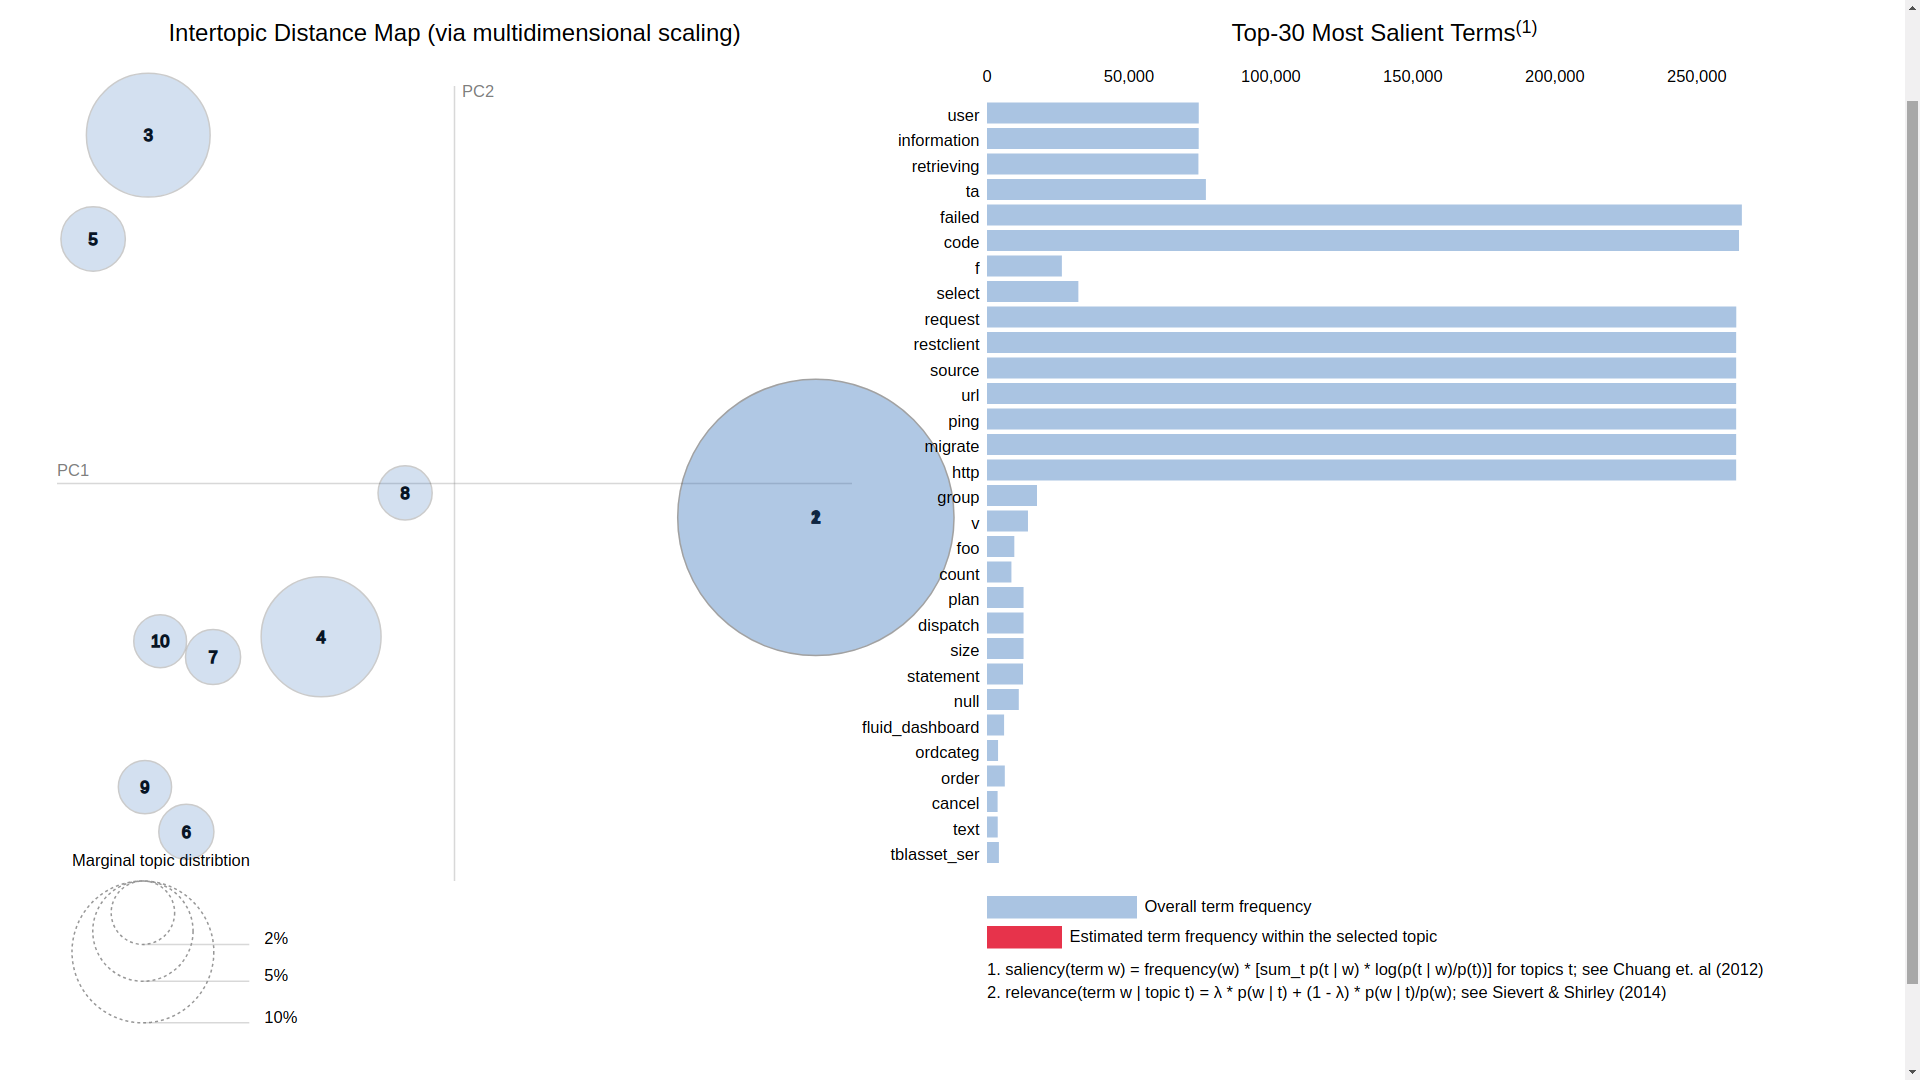
\includegraphics[width=15cm, height=8cm,trim=0 0 100px 0, clip=true]{figures/pyldavis/pyldavis_10.png}
    \caption{PyLdavis topic visualisation with 10 topics}
    \label{fig:pyldavis_10}
\end{figure}

In Fig \ref{fig:pyldavis_10} we jump to 10 topics. Closer inspection of the pyLDAvis shows overlap in topic 1 and 2. The remaining topics are reasonably well distinguished and show no overlap. 

Further examining the remaining figures we like to state the following:
\begin{enumerate}
  \item The remaining figures show no clear preference of topic count
  \item The majority of figures appear to have overlapping topics
\end{enumerate}
The first statement is probably because pyLDAvis is created to help show a global topic distinctiveness but also help the user interpret the topics relevant term. This means it is not necessarily built for different topic count comparison. The second statement is once again due to the nature of LDA which has overlapping terms in different topics, like the topics in 1 and 2 in the 10 topics model.

\FloatBarrier
\section{Coherence}\label{results:coherence}
The next results show a topic coherence score in correlation to topics count. Our Fig \ref{fig:coherence} shows the average value each model scored. 

The results in the topic coherence show interesting scores. Moreover, it is surprising and interesting that the coherence values shown fluctuate a lot The scores are peaking at 11 topics and having its lowest score at 35 topics. Most score between 3 and 20 show an above average score on coherence. Topic 23 the second highest coherence score. 

 \begin{figure}[h]
    \centering
    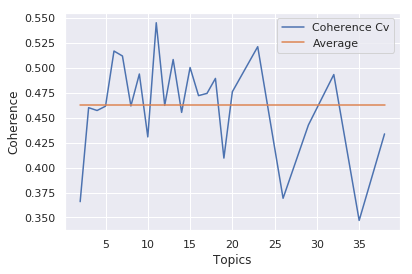
\includegraphics[width=15cm, height=8cm]{figures/coherence_values_topics.png}
    \caption{Coherence values based on the measure Cv}
    \label{fig:coherence}
\end{figure}

\FloatBarrier
\section{Document distribution based on hard clustering}\label{results:doc_distribution}
Fig \ref{fig:doc_distr_1-11corpus} and Fig \ref{fig:doc_distr_1-11held_out} represent the count of documents in their respective highest probable topic. 

When looking at both the figures we notice similar distribution. Furthermore, interestingly enough our results show 3 dominant topic counts. 

\begin{figure}[h]
    \centering
    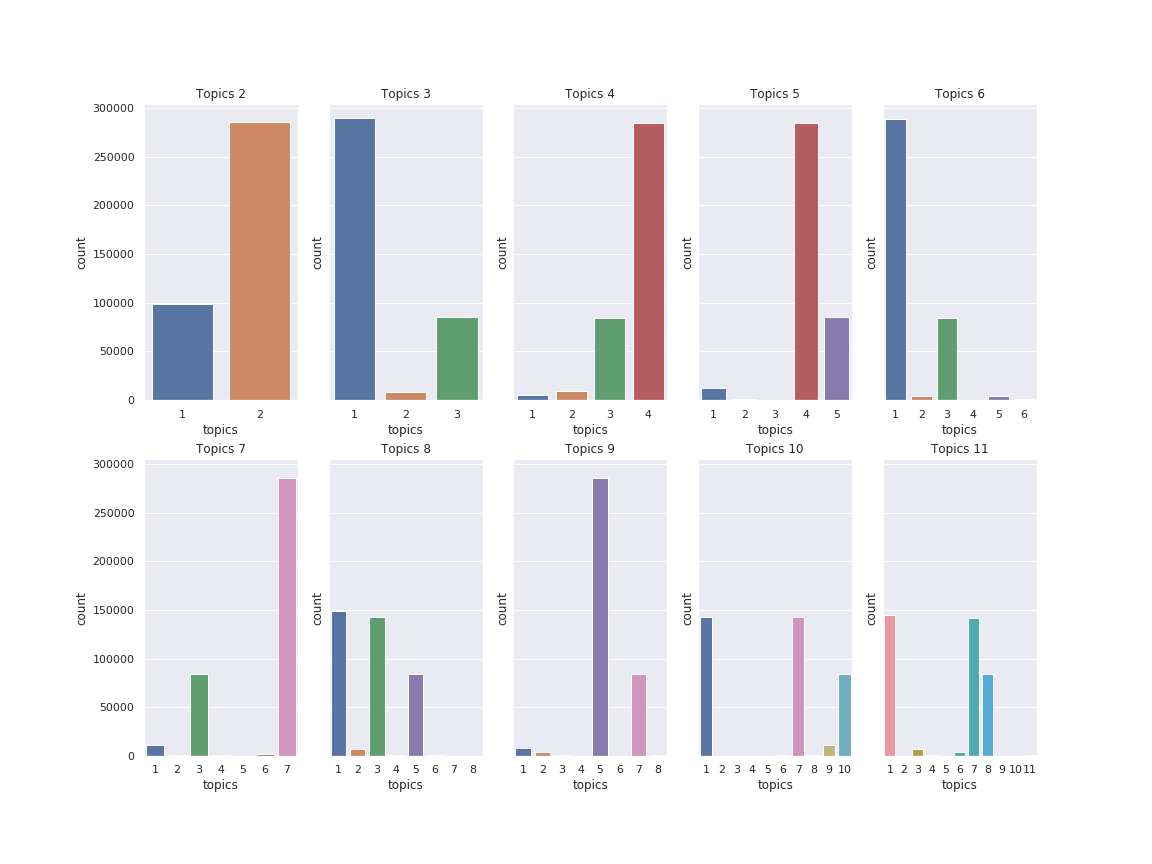
\includegraphics[width=16cm, height=12cm]{figures/doc_distr/doc_distribution_1-11_corpus.png}
    \caption{Document distribution on the train test data}
    \label{fig:doc_distr_1-11corpus}
\end{figure}

Inspecting Fig \ref{fig:doc_distr_1-11corpus} we notice the figure has a lot of empty topic clusters. Again this is expected based on the skewed form of the terms in earlier exploration of the data. The interesting fact is that most documents can be clustered into 3 topics. 

\begin{figure}[h]
    \centering
    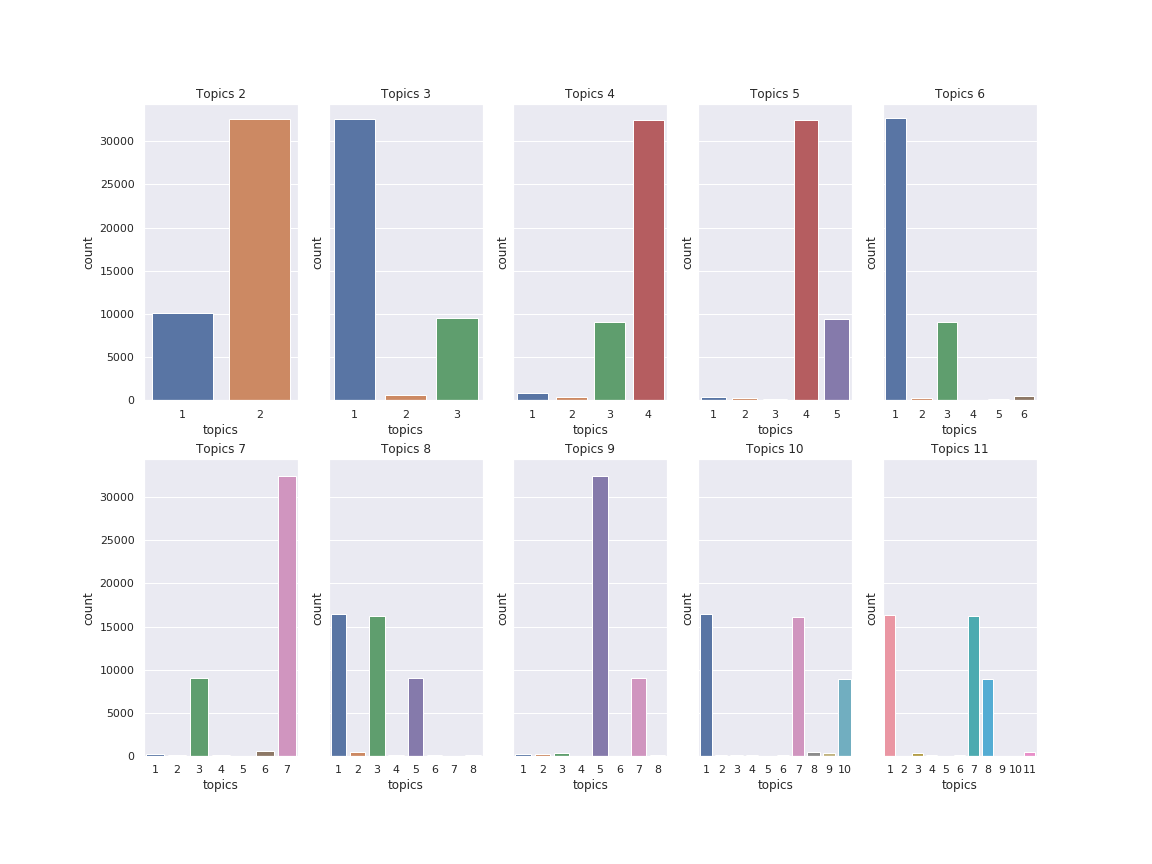
\includegraphics[width=16cm, height=12cm]{figures/doc_distr/doc_distribution_1-11.png}
    \caption{Documents distribution on the held out data}
    \label{fig:doc_distr_1-11held_out}
\end{figure}

The same can be repeated for Fig \ref{fig:doc_distr_1-11held_out}. Although the held out data is created after shuffling the data and then splitting it, the distribution of documents in each cluster for each model is remarkably similar. 

The remaining document clustering are in the appendix A. As we suspect the models show similar document distribution in held out compared to train and test data. The results do differ in document distribution, which so far were primarily in 3 topics. The increasing amount of topics does show increasing amount of topics with similar sizes. This occurrence is probably simply due to dominant and large topics being split in multiple topics.

\FloatBarrier

\section{Silhouette values}\label{results:silhouette}
The final metric we evaluate with is the cosine metric. Our held out and train and test data are sampled on 10000 documents and hard clustered based on their highest probable topic. After 13 topics the silhouette values can not be calculated anymore. The mathematical explanation is that the denominator has a value of zero, as such it can not calculate the silhouette of a sample. This means that topics have become so small and overlapping that the average distance for each sample in a cluster and the nearest cluster has become 0.

\begin{figure}[h]
    \centering
    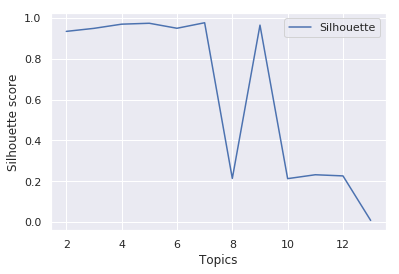
\includegraphics[width=15cm, height=8cm]{figures/silhouette_values_topics_corpus.png}
    \caption{Silhouette values based on the train test data}
    \label{fig:Train test dataset}
\end{figure}

The silhouette values for each topic is constantly high, suddenly being drastically lower at topic 8 and after topic 9. Silhouette values show the inter and intra cluster relationship and while the topics might be infered to be good when compared to each other based on the coherence, silhouette shows us that the documents still have a hard time to be properly clustered after a certain amount of topics on our dataset.

\begin{figure}[h]
    \centering
    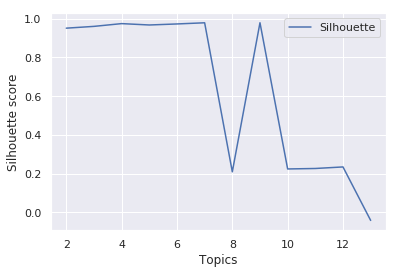
\includegraphics[width=15cm, height=8cm]{figures/silhouette_values_topics_held_out.png}
    \caption{Silhouette score based on the held out data}
    \label{fig:Held out}
\end{figure}

Similar scores are achieved on our held out dataset. The results from the held out are similar enough, so we might say that the expectation of our models align with the expectation further. 

\FloatBarrier
\section{Contribution}\label{results:contribution}
In this section we will discuss the findings from our research. These findings include the data extraction and exploration of server logs. Applying the online LDA model on the dataset and the general difficulty of evaluating the models. 

The data extraction has been interesting, having access to such a huge amount of data for exploration is a treat for every researcher. Earlier research has been performed on extracting server logs for analyses, but not a lot of research is performed using this huge amount of data. Our data can be said to be unique in the aspect of having no labels, which most researchers depend heavily on.

As such we found the LDA machine learning model suitable to provide our dataset with the necessary structure for our dataset. Unsupervised machine learning on server logs through document mining has not been done with much success or without much effort in the past.

The nature of LDA, makes it hard to evaluate correctly because LDA can be evaluated using metrics which show to have a good performance for extracting latent topics which humans can recognise. The nature of this dataset once again is that humans can not understand it easy, except maybe if one is a domain expert. Continuing with this knowledge we were interesting at the semantic analyses which LDA could provide.

The results shown in our chapter \ref{ch:results}, show interesting results and even contradicting results. The latent topics infered were evaluated on distinctiveness and coherence. We took a brief look in section \ref{results:topics} of our topics with their terms and experienced the difficulty hands on of interpreting these topics and choosing the optimal number of topics. Following we use pyLDAvis, which is widely used for topic distinctiveness interpretation and easy interpretation of topics itself. Furthermore we evaluated the coherence of topics with coherence metric Cv.

Finally we chose to hard cluster the documents in their most probable topics using the silhouette coefficient to see that similar documents are indeed clustered together for certain amount of topics, corresponding with our held out dataset for final confirmation of the quality.

We will discuss the final conclusion drawn from our experiments and answer the general research question in the conclusion next chapter.

\begin{comment}
I dont think I contributed a lot to the research in this area, but I learned a lot right??
\end{comment}
